%% MISSCHIEN NOG TOEVOEGEN:
%Hoe verschilt ons data van text documenten?
%To make use of this method a suitable feature representation of the available data is required. The features are found by counting the activations of sensor groups. In this way a relative low number of dimensions are found, which can contain positive integers. In theory these numbers have an infinite range, but in practice the count of sensor activations of every dimension is reduced to a maximum.\\
%This feature representation differs a lot to the Bag-of-words model that is often used for the description of textual data. In this representation a dictionary of all possible words is build and a document can be described with a binary vector of the same length as the size of the dictionary. With respect to our data, text data thus has much more dimension but every dimension only contains a binary value.




In the first section of this chapter the general idea of topic models is introduced. This section is followed by a description of how this kind of models can be applied the sensor data. After that the extension of the LDA model 'LDA-Gaussian' is given, including the EM-algorithm that is used to determine the model parameters. This chapter is finalized with the description of the LDA-Poisson model.

\section{Introduction to Topic Models}
Topic models are often used in the field of document classification. Given a set of documents (corpus) it is assumed that every document belongs to one or more topic(s). So for example a news article may belong for some percentage, let us say 30 \%,  to the topic 'Economy' and for 70 \%  to the topic 'Politics'. Another document of the same Corpus may belong to the topic 'Economy' with 50 \%, 'Politics' with 30 \% and 'Finance' with 20 \%. There might be a lot of different topics and the topics can have different level of details. \\
The topics are defined by several words that can occur in the documents. The topic 'Economy' may be defined by the list of words \{'trade', 'industry','GDP'\}. Other topics have different lists of words that describe them. The list might be longer or shorter and the words in the list will depend on the corpus that is used to generate the topics. It might also be the case that one word belongs to multiple topics. Eventually we can find the topic distribution of a document according to the words that are included in this document.\\
In the topic model 'Latent Dirichlet Allocation' (LDA) it is assumed that a Corpus can be made out of a generative process. The parameters that generate the corpus are than used to describe the model of the corpus. The generative process which builds a corpus is as follows:\\
For every document that is generated in the Corpus
\begin{enumerate}
 \item Choose the amount of words in the document from $N \sim Possoin(\xi)$.
 \item Choose a topic distribution $\theta \sim Dir(\alpha)$ for the document.
 \item For each of the N words $w_n$:
 
 \begin{enumerate}
  \item Choose a topic $z_n \sim Multinomial(\theta)$.
  \item Choose a set of words $w_n$ from the set of all words $V$ from $p(o_n |z_n;\beta)$, a multinomial probability conditioned on the topic $z_n$. Where $\beta$ is the distribution over words given a topic.
 \end{enumerate}

\end{enumerate}

The model is also shown in figure~\ref{fig:modelBasic}. The parameters $\alpha$ and $\beta$ define a corpus.

\begin{figure}[h!]
\centering
\def\svgwidth{400pt}
\input{Pictures/ModelBasic.pdf_tex}
\caption{Graphical representation of the LDA model}
\label{fig:modelBasic}
\end{figure}

To determine the model parameters an EM-algorithm can be used. How this algorithm can be applied is extensively described in~\cite{blei2003latent}. \\
In the next section it is described how this model can be used with the sensor data, that is gained in the different houses.


\section{Topic models with Sensor Data}

In order to employ the topic model with the sensor data, first the different levels of description are introduced and relate to the terms of document classification.
\begin{itemize}
 \item \textbf{Dataset/Corpus}: One dataset $C$ describes the sensor data that is obtained in the home of a single person. So for every person there is a separate dataset. This set of data can be compared with a Corpus in document classification.
 \item \textbf{Day/Document}: Every dataset is divided in days, which is a natural choice because daily routines are a good indication for behavior patterns. A day can be compared with a document in a Corpus.
 \item \textbf{Observations/Words}: Finally every day is build of a set of observations, which are already introduced in chapter \ref{chapter:features}. Observations can be roughly compared with words in document classification. A different name for this observations is  'Artificial words'.
\end{itemize}

There are some differences between the data that is used for topic detection in text documents and in data obtained from binary sensors.\\
The main difference is that words that look similar to each other, like "illusion" and "allusion", may belong to a totally different topic in the document classification. But in the case of sensor data, two observation that are similar to each other, are more likely to refer to the same topic. So for example if the topic "preparing breakfast" has the observation $o_n = {2,4,0,3,2,2}$ a similar observation like $o_n={2,4,0,4,2,2}$, where only the fourth value of the vector is changed, may also refer to the same topic. With a BOW model, where every unique observation forms a new dimension, this similarity cannot directly be captured. The only way to capture this relationship is by observing the similar observations with another observation. Say observation A and B are similar to each other. So if observation A is seen with observation C and also B is seen with C, then it might be possible that the LDA algorithm assigns the same topic for A and B. A lot of data is necessary to find these kind of relations.\\
Another difference is that in the topic model LDA, it is assumed that the order of the words in the text is not important. However with sensor data the time when an observation is made is of big influence. By adding the time value to the observation we can overcome this problem. The fine grain time representation (see chapter \ref{chapter:features}) will contain more information about the sequential order of the observations than the coarse grain representation.\\





% Plaatje a) omschrijven
If the Bag-of-Words model will be applied to the data, a dictionary of all unique observations must be made. All this observations then can be seen as a different dimension which are independent of each other. In figure~\ref{fig:FSBOW} an example is shown how a topic model can assign topics to the different observations. It is not necessary that two observations lay close to each other if they are assigned to the same topics. So the spatial relationship between the observation is not taken into account. Observations can be assigned to multiple topics.\\
\begin{figure}[h!]
\centering
\begin{minipage}[b]{0.3\linewidth}
\centering
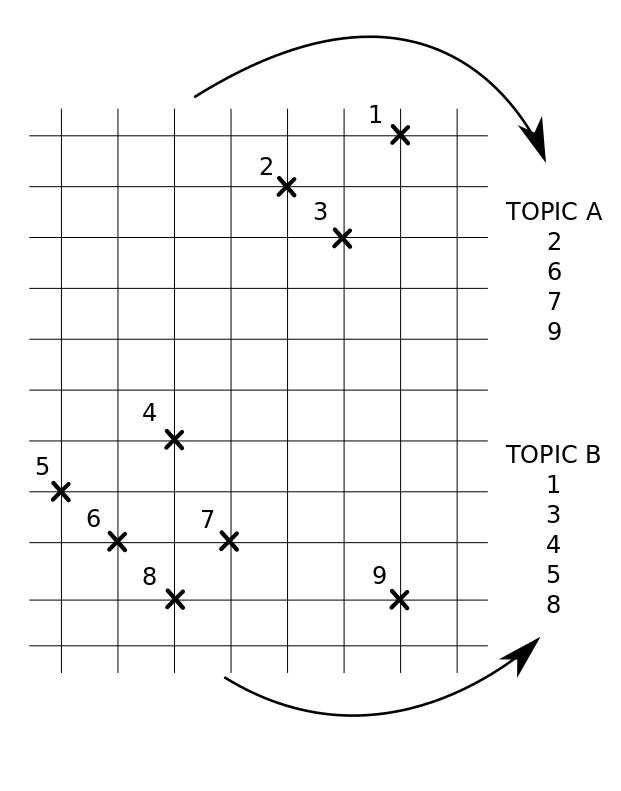
\includegraphics[width=\textwidth]{Pictures/BOW.png}
\caption{The Bag-of-words model with topic assignment.}
\label{fig:FSBOW}
\end{minipage}
~
\begin{minipage}[b]{0.3\linewidth}
\centering
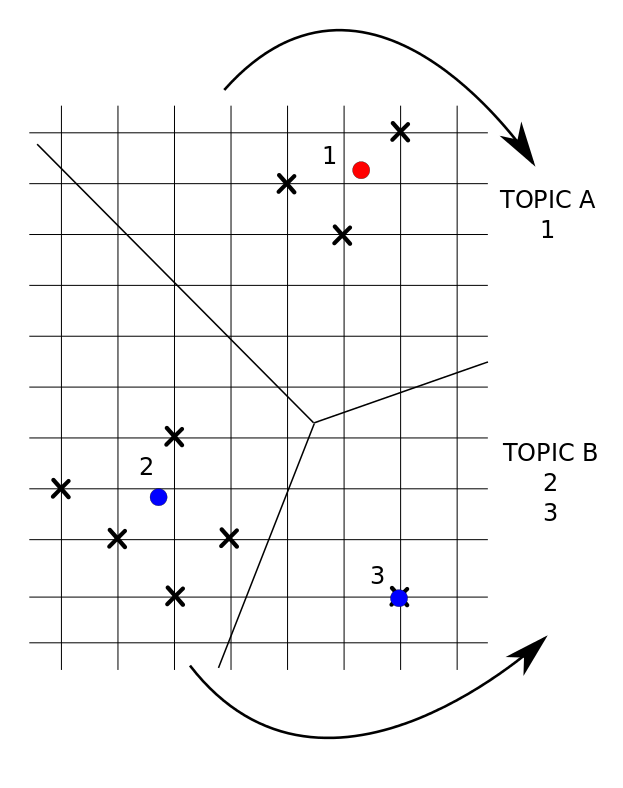
\includegraphics[width=\textwidth]{Pictures/kMeans.png}
\caption{Feature space with k-means and topic assignment.}
\label{fig:FSk-means}
\end{minipage}
\end{figure}

\begin{figure}[h]
\centering
\def\svgwidth{140pt}
\input{Pictures/GMM.pdf_tex}
\caption{Gaussian Mixture Model with LDA. Topic A is marked with red. Topic B is marked with blue (clustering on forehand with GMM) and with green (combination of GMM and LDA)}
\label{fig:GMM+LDA}
\end{figure}

% plaatje b) omschrijven
To make sure that similar observations will be grouped together and appear in the same topic, the k-means algorithm can be applied to find clusters in the data. The id's of the centroids of the clusters then function as the 'artificial words'. The size of the dictionary of the BOW model is in this way reduced. Applying LDA on this reduced representation can lead to a better topic description. This is shown in figure \ref{fig:FSk-means}.\\
% plaatje c) omschrijven
The outcome of the LDA model does strongly depend on the outcome of the apriori used cluster algorithm. Choosing the correct amount of clusters for the k-means algorithm can be difficult, as it is also pointed out in the work of Casale \cite{Casale:2009}. And still it can occur that the clusters do not give a good representation of the data. All clusters have the same influence on the LDA model, which is not always desirable. A Gaussian Mixture model (GMM) can give a better description of the clusters and give a degradation of the topics. Every Gaussian distribution can be assigned to a topic with the LDA model. This is shown in figure \ref{fig:GMM+LDA} with the red and blue Gaussian distributions. The red distribution is assigned to one topic and the two blue distributions are assigned to another topic.\\
Combining the clustering and the Topic model directly together can lead to a more global representation of the topics. This is indicated with the green Gaussian distribution in the figure, which combines the two blue distribution into one. 



 

% With a Gaussian Mixture Model it might be possible to distinguish between more or less important clusters. But we might want to let the topic model decide which topics have more influence and which have not, according to the data.\\
% That is why we combined the clustering part and the topic estimation into one step. Instead of a multinomial distribution over all observations that occur in the 'Dictionary', we model a Gaussian distribution over every dimension of the observations. In this way similar observation can be captured in the model itself and are not generalized in one cluster beforehand.\\
% The difference is that instead of a large, fixed set of unique observations (Dictionary), with a multinomial distribution, we take a Gaussian distribution over every dimension of the observations. In this way unseen observations will be handled properly.
% In the next sections we describe the model in more detail. We first give an overview of the generative process. Then we explain the variational inference that is necessary to make the parameter estimation possible. And finally explain the EM-algorithm that determines the parameters.
% 


% 
% Let us say we have a two dimensional feature space. For example we only have two sensors in our data, than every dimension will refer to one of the sensors. A representation of this model is shown in figure bla (a). A cross marks an observation and is seen as a new 'word' in the bag-of-word method. We can use this data with the LDA model. The problem only with this approach is that similar observations are not group together and it might be possible that a similar observations are not grouped together in the same topic when we apply the LDA model.

% 
% 
% If we cluster the observations on forehand with a the k-means algorithm we can reduce the size of the dictionary (which contains all unique observations) and use again the LDA method to find the topics. The problem here is that there is a hard separation line between the clusters as is shown in figure bla (b).
% 
% So we invented a third method which is a kind of gaussian mixture model included into the LDA topic model. So instead of cluster the model with priors from the data itself we relate the priors directly to the topis and combing the part of clustering and the deriving the topics in one algorithm. In this way clusters are grouped together directly if they belong to the same topic, as is shown in figure bla (c).
% 
% 
% 

% 
% 
% In the next two sections we describe the two different ways how we use the topic models with our data. First we describe the combination of k-means clustering and the basic LDA model as it is described in [Blei]. And after that we describe our new approach that combines the clustering and topic modelling in one algorithm. In this algorithm we step away from the bag-of-words model representation of the data.
%  Nog toevoegen dat we twee manieren gaan gebruiken(LDAbasic and LDAext)
% %%TOT HIER!
% 
% 

%   \subsubsection{K-means}
%  In the previous section we addressed the problem of a wide variance of observations. With a bag-of-words model, as it is used in the LDA approach, similar looking words/observations are not likely to be put in the same topic. All observations, that are not exactly the same, are independent from each other and may not lead to the same topic. Because of the low amount of training data it is not very likely that the same observation will be seen often enough to learn topics from the data properly.
% That is why we need to reduce the amount of unique observations and group similar observations together. In terms of document classification, we could say that we need to reduce the size of the dictionary.


% In a first-approach we use k-means clustering to reduce the size of the dictionary, which is the set of all observations that can be found in the data.
% We do not use the time dimension for the clustering part, because this would compromise our data so that clusters are not detected properly. We use the euclidean distance to determine the best mean.
% 
% maybe preprocess the data with coarse grain time dimension
% 
% size of the dictionary
% is it the case that with a lot of data simialar looking words will be put in the same topic? Or will it just be a different topic?
% 
% 
% 
% In our data the size of the dictionary, which contains all unique observations in the whole corpus is relative large with respect to the size of the data that we have. There are a lot of different observations that are similar to each other, but differ only in one value of the 6 dimensions. So for example the observation $o_1=\{1 ,2 ,5 ,3,14\}$ is similar to the observation $o_2=\{2 ,2 ,5 ,3,14\}$. The only difference of sensor activities is in the first field. In the LDA model these two observations/words will be seen as two different dimensions and the similarities are not captured. In fact a lot of words will only be seen once in the whole corpus and finding good parameters is not possible.
%  So we need to find a way to capture similar observations to build a proper topic model. A simple way is to cluster all observations together and then use the EM-algorithm to estimate the parameters of the  LDA model.
%  For the clustering part we used the k-means algorithm. We reduced the size of the dictionary to 20. After that we use the EM-algorithm as described above.
%  In the clustering we leave out the time dimension because this is fucking up the clusters
 
%   \subsubsection{Latent Dirichlet Allocation with clustered Data}
% The generative model 'Latent Dirichlet Allocation' [Blei] is a way to describe a topic model. In this model it is assumed that a Corpus can be generated from a distribution of topics, where every topic can be represented with a distribution of words. In our case the documents are days and the words are observations $o_n$. In the previous section we described how we reduced the size of the dictionary $V$.
% The generative process that would create the data will look like this:
% 
% For every day that will be generated:
% \begin{enumerate}
%  \item Set the amount of observations in every document to size N (for every day the same amount).
%  \item Choose a topic distribution $\theta \sim Dir(\alpha)$ for the day.
%  \item For each of the N observations $o_n$:
%  
%  \begin{enumerate}
%   \item Choose a topic $z_n \sim Multinomial(\theta)$.
%   \item Choose a set of observations $o_n$ from the set of all observations $V$ from $p(o_n |z_n;\beta)$, a multinomial probability conditioned on the topic $z_n$. Where $\beta$ is the distribution over observations given a topic.
%  \end{enumerate}
% 
% \end{enumerate}
% %!!!Describe the model variables!!!!!
% 
% With the assumption that the data that we got from the sensor system has the same structure than the data created with the generative process we can find the model parameters $\alpha$ and $\beta$ for LDA with the EM-algorithme described in \cite{blei2003latent}.

\section{LDA-Gaussian Model}
In this section the LDA-Gaussian model is described. First the model is explained, which is followed by the description of the variational inference. This inferense step is necessary to calculate the model parameters. In this subsection also the two steps of the EM-algorithm are explained.



% Every topic will have its own distribution over the dimensions. A
% topic can be described as shown in figure %\ref{fig:topic}.
% In this figure an example of a topic description is shown
% \begin{figure}
%  \includegraphics[\width=\textwidth]{Pictures\topics.png}
%  \caption{An awesome topic}
%  \label{fig:topic}
% \end{figure}

  \subsection{Model Description}
  
  For the model it is assumed that every day in a dataset can be represented as random mixture of latent topics, where every topic can be described as a distribution over observations. The following generative process is assumed for every day $m$ in the data set $C$:
\begin{enumerate}
 \item The amount of observations on a day $m$ is fixed with size $N$ (for every day the same size).
 \item A day has a distribution over the topics given with $\theta \sim Dir(\alpha)$.
 \item For each of the N observations on a day $o_n$:
 
 \begin{enumerate}
  \item Estimate the topic $z_n \sim Multinomial(\theta)$.
  \item An observation $o_n$ is gained from $p(o_n |z_n,\boldsymbol\mu,\boldsymbol\sigma)$,  which is a probability that can be drawn from a set of Gaussian distributions. This probability is conditioned on the topic $z_n$ and the Gaussian Parameters $\vec{\mu_i}$ and $\vec{\sigma_i}$ of length $d$ that belong to the estimated topic $i=z_n$.
 \end{enumerate}

\end{enumerate}
  
In this model the amount of topics $k$ is assumed to be known and fixed and with it the size of the topic variable $z$.
The probability for the observations is parametrized with two matrices $\boldsymbol\mu$ and $\boldsymbol\sigma$, both of size $D\times k$, where $D$ is the amount of dimensions in an observation and $k$ the amount of topics. They present the mean and standard deviation respectively and for every topic $i$ and every dimension $d$ there is a set of parameters, which describes a Gaussian distribution. Every value of a dimension for an observation $o_{ndi}$ can then be drawn from a Gaussian Distribution $\mathcal{N}(\mu_{di},\sigma_{di})$.\\
With the feature representation given in chapter \ref{chapter:features} the size of the dimension is fixed with $D=6$. $\alpha$ represents the Dirichlet parameter and is vector of length $k$.

In figure \ref{fig:modelExt} the graphical representation of the model is shown. It differs from the basic LDA model (figure \ref{fig:modelBasic}) in the description of the topic distribution $\beta$, which is here replaced with $\mu$ and $\sigma$.

\begin{figure}[h!]
\centering
\def\svgwidth{0.8\textwidth}
\input{Pictures/ModelExt.pdf_tex}
\caption{Graphical representation of the LDA-Gaussian model}
\label{fig:modelExt}
\end{figure}




  
Assuming that the generative process described above can describe the available data properly, the optimal parameters need to be found. Therefore the probability for the dataset $C$ needs to be maximized, with respect to the parameters $\alpha$, $\mu$ and $\sigma$.
This probability looks like this
\begin{equation}
p(C|\alpha,\mu,\sigma) = \prod_{m=1}^M p(m|\alpha,\mu,\sigma)
\end{equation}
where $M$ is the amount of days within the dataset and the probability for a day $m$ given the three parameters, which is the marginal distribution over a day, is
\begin{equation} 
p(m|\alpha,\mu,\sigma) = \int p(\theta|\alpha)  \left( \prod_{n=1}^N \sum_{z_n} p(z_n|\theta) p(w_n|z_n, \mu,\sigma)  \right) d\theta
\end{equation}
This distribution is obtained by integrating the joint distribution \ref{eq:Joint} by $\theta$.
\begin{equation} \label{eq:Joint}
 p(\theta,\textbf{z},\textbf{w}|\alpha,\mu,\sigma) = p(\theta|\alpha) \prod_{n=1}^N p(z_n|\theta) p(w_n|z_n,\mu,\sigma)
\end{equation}
In the next section it is described how the optimal parameters for the model given a data set can be found.


  
\subsection{Variational Inference}
 
The marginal distribution, which is given in the previous section, can be written in terms of the parameter $\alpha$, $\mu$ and $\sigma$ as
  \begin{equation}
   p(m|\alpha,\mu,\sigma) = \frac{\Gamma (\sum_i \alpha_i)}{\prod_i \Gamma(\alpha_i)} \int \left( \prod_{i=1}^k \theta_i^{\alpha_i-1} \right)
   \left( \prod_{n=1}^N \sum_{i=1}^k \prod_{d=1}^D \theta_i \mathcal{N}(o_{nd},\mu_{id},\sigma_{id} ) \right)
  \end{equation}
Due to the coupling between $\theta$ and the Gaussian parameters $\mu$ and $\sigma$ this probability is intractable to compute.	




That is why a convexity-based variational algorithm is applied, so that the log-likelihood of a given dataset can be approximated. 
An approximation of the model is given with 
  \begin{equation}
   q(\theta,z|\gamma,\phi) = q(\theta|\gamma) \prod_{n=1}^N q(z_n|\phi_n).
  \end{equation}
In this model $\gamma$ represents the Dirichlet parameter and $\phi$ are the multinominal parameter which can be viewed as the probability $p(z_i|o_n)$ and is given as a $k \times N$-matrix for every day $m$. The graphical representation of the model is shown in figure \ref{fig:ModelApprox}.
  
 
\begin{figure}[h!]
\centering
\def\svgwidth{0.4\textwidth}
\input{Pictures/approxModel2.pdf_tex}
\caption{Approximation of the model.}
\label{fig:ModelApprox}
\end{figure}
 
  
  
  
  Given the variational distribution for the approximate model the lower bound of the log-likelihood can be estimated with the Jensen inequality
  \begin{equation}
   \begin{split}
    L(\gamma;\phi;\alpha;\mu;\sigma) =& E_q[\log p(\theta|\alpha)] + E_q[\log p(\textbf{z}|\theta)] + E_q[\log p(\textbf{w}|\textbf{z},\mu,\sigma)] \\
   & -E_q[\log p(\theta)] - E_q[\log q(\textbf{z})]
   \end{split}
  \end{equation}

In terms of the model parameters and the variational parameters this becomes
\begin{equation}
  \begin{split}
 L(\gamma;\phi;\alpha;\mu;\sigma) =& \log \Gamma (\sum_{j=1}^k \alpha_j) - \sum_{i=1}^k \log \Gamma(\alpha_i) + \sum_{i=1}^k (\alpha_i-1)(\Psi(\gamma_i)-\Psi(\sum_{j=1}^k \gamma_j)) \\
 & + \sum_{n=1}^N \sum_{i=1}^k \phi_{ni} (\Psi(\gamma_i)-\Psi(\sum_{j=1}^k \gamma_i)) \\
  & + \sum_{n=1}^N \sum_{i=1}^k \sum_{d=1}^D \phi_{ni} \log( \mathcal{N}(o_{nd};\mu_{id},\sigma_{id})) \\
  & - \log \Gamma (\sum_{j=1}^k \gamma_j) + \sum_{i=1}^k \log \Gamma (\gamma_i) - \sum_{i=1}^k (\gamma_i -1)(\Psi(\gamma_i)-\Psi(\sum_{j=1}^k \gamma_j)) \\
 & - \sum_{n=1}^N \sum_{i=1}^k \phi_{ni} \log \phi_{ni}
  \end{split}
  \label{eq:likeli}
\end{equation}

An EM-process is able to maximize this lower bound on the log-likelihood. The two steps are:
  \begin{enumerate}
   \item \textbf{E-step:} For each day $m$, optimize the variational parameters $\{ \gamma_{m}*,\phi_{m}* \}$
   \item \textbf{M-step:} Maximize the resulting lower bound on the log-likelihood with respect to the model parameters $\alpha$, $\mu$ and $\sigma$.
  \end{enumerate}
  
  Now a more detailed description on both of these steps is given:
  
  \paragraph{E-step}
In the E-step of the algorithm the variational parameters $\phi$ and $\gamma$ are optimized. To get the update function for $\phi$ all terms of the lower bound of the log-likelihood in equation (\ref{eq:likeli}) are gathered, that contain the variable $\phi$. 
Take $y_i=\sum_{d=1}^D \mathcal{N}(o_{nd};\mu_{id},\sigma_{id})$ and add the constraint $\sum_{i=1}^k \phi_{ni}=1 $ . This results in the following formula
\begin{equation}
 L_{[\phi_{ni}]} = \phi_{ni}(\Psi(\gamma_i)-\Psi(\sum_{j=1}^k \gamma_j)) + \phi_{ni} \log(y_i) + \lambda_n(\sum_{j=1}^k \phi_{ni} -1)
\end{equation}
From this equation the derivative can be taken and set it to zero. This leads to the first update function
\begin{equation}
 \phi_{ni} \propto \log(y_i) \exp(\Psi(\gamma_i) - \Psi(\sum_{j=1}^k \gamma_j))
\end{equation}\\

A similar approach is handled for $\gamma$. Again all terms of equation \ref{eq:likeli} that contain this variable is selected and the derivative is set to zero. This leads to the second update equation
\begin{equation}
 \gamma_i = \alpha_i + \sum_{n=1}^N \phi_{ni}
\end{equation}

  %Nu nog de algorithme geven

  \paragraph{M-Step}
  
In the M-step the parameters of the Gaussian distribution $\mu$ and $\sigma$ are estimated with the weighted arithmetic mean calculated over all observation in a dataset given the parameter $\phi$, which is gained in the previously e-step. This leads to the update formulas
\begin{equation}
 \mu_{di} = \frac{\sum_{m=1}^M \sum_{n=1}^N o_{dn} \phi_{ni} }{\sum_{m=1}^M \sum_{n=1}^N  \phi_{ni}}
\end{equation}
and
\begin{equation}
 \sigma_{di} = \sqrt{\frac{\sum_{m=1}^M \sum_{n=1}^N o_{dn}^2 \phi_{ni} }{\sum_{m=1}^M \sum_{n=1}^N  \phi_{ni}} - \mu_{di}^2}
\end{equation}\\

To calculate the parameter $\alpha$ again all terms of the likelihood that contains the variable $\alpha$ are selected. The derivative in the Hessian form is
\begin{equation}
 \frac{\partial L}{\partial \alpha_i\alpha_j} =  m(i,j) M \Psi'(\alpha_i) - \Psi'(\sum_{j=1}^k \alpha_j)
\end{equation}
On this equation the Newton-Rhapson method can be used to calculate the optimal $\alpha$.

\section{LDA-Poisson Model}

The feature description in chapter \ref{chapter:features} generates positive integers. Small values are more likely to occur in the observations and that is why a Poisson distribution is a better choice for the description of the topics. In figure \ref{fig:LDAPoisson} the graphical representation of LDA-Poisson model is shown. 

\begin{figure}[h!]
\centering
\def\svgwidth{0.8\textwidth}
\input{Pictures/ModelPois.pdf_tex}
\caption{Graphical representation of the LDA-Poisson model.}
\label{fig:LDAPoisson}
\end{figure}

The variational Inference and the EM-procedure will be the same as described before, except for the Gaussian distribution that is exchanged with the Poisson distribution. The parameter $lambda$ which describes the Poisson distribution is calculated in the M-step with
\begin{equation}
 \lambda_{di} = \frac{\sum_{m=1}^M \sum_{n=1}^N o_{dn} \phi_{ni} }{\sum_{m=1}^M \sum_{n=1}^N  \phi_{ni}}.
\end{equation}



% For a reason 
% the reason is that lda captures priors for the days, that are given with the 
% which is still not is clear for me, we combine the clustering and determining of the topics in one algorithm.
% Preprocessing the data with k-means may not capture the topic distributions probably. The time dimension is not taken into account in the clustering part. So we want to avoid the preprocessing the data with k-means and add the the clustering part directly in the model.
% So first we describe how the model will change with respect to the LDA model descriibed above (or maybe: ... how extension of the LDA model looks like) and we also describe how the parameters are determined with the EM algorithm.
% 
% 
% So what is different? Maybe do not ask this question but just explain how the model looks like.
% 
% The main change of the model is that it is also captures similar observation in one topic.
%  So instead of describing a topic only with one discrete value in one dimension, we model every dimension in the observation with a Gaussian distribution. So every dimension given a topic needs to be defined with a mean and a standard deviation. The dimension might depend from each other
% 
% 
%   This is done in the following way:
% Instead of storing the probability for a observation given a topic, which is done in the matrix $\beta$, we assume that every dimension of the observations is normal distributed given a topic. So we store the mean and variance for every dimension given a topic in two matrices of size $d \times k$ where $d$ is the dimension of the observations and $k$ the amount of clusters. For now we assume that the dimensions of the observations are uncorrelated. The EM-algorithm is adjusted to calculate the $\beta$- matrix properly.
% 
% - The combination of the k-means clustering and the LDA model might not capture the topics correctly. The k-means clustering gives a hard boundaries on the words, which is also a drawback from the sequential combination of clustering and topic estiamtion. Therefore we want to comine these two step in one.
